\subsection{Settings}
\begin{frame}[noframenumbering]{Table of Contents}
  \tableofcontents[currentsection, currentsubsection]
\end{frame}


\begin{frame}
  Let $\Omega = (-1,1)^2$. Define $f\in H^1_0(\Omega)$ by 
  $f(x)=\tilde{f}(|x|)$ for all $x\in\Omega$ with
  \begin{align*}
    \tilde{f}(r)\coloneqq 
    \begin{cases}
      \alpha-12(2-9r) & \text{if } 0\leq r\leq\frac{1}{6},\\
      6r\alpha-\frac{1}{r} & \text{if } \frac{1}{6}\leq r\leq
      \frac{1}{3}\\
      2\alpha+6\pi\sin(\pi(6r-2))-\frac{1}{r}\cos(\pi(6r-2)) &
      \text{if } \frac{1}{3}\leq r\leq\frac{1}{2},\\
      \alpha(5-6r)+\frac{1}{r}&
      \text{if } \frac{1}{2}\leq r\leq\frac{5}{6},\\
      -3\pi\sin(\pi(6r-5))+\frac{1+\cos(\pi(6r-5))}{2r} &
      \text{if } \frac{5}{6}\leq r\leq 1.
    \end{cases}
  \end{align*}
  
  \begin{figure}[!ht]
    \centering
    \begin{subfigure}{.4\linewidth}
      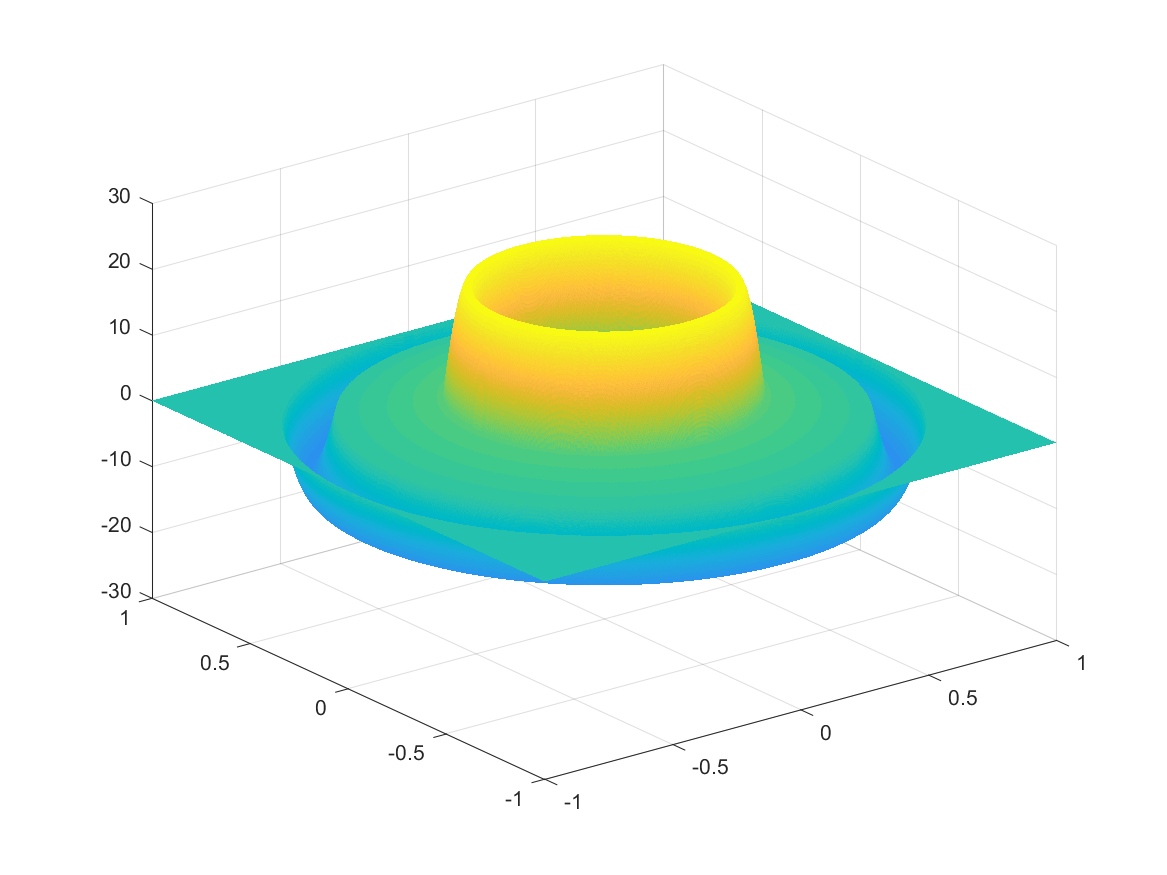
\includegraphics[width=\linewidth]
        {pictures/experiments/settings/f01/rhs.png}
      \caption*{$f$ for $\alpha=1$}
    \end{subfigure}
    \quad
    \begin{subfigure}{.4\linewidth}
      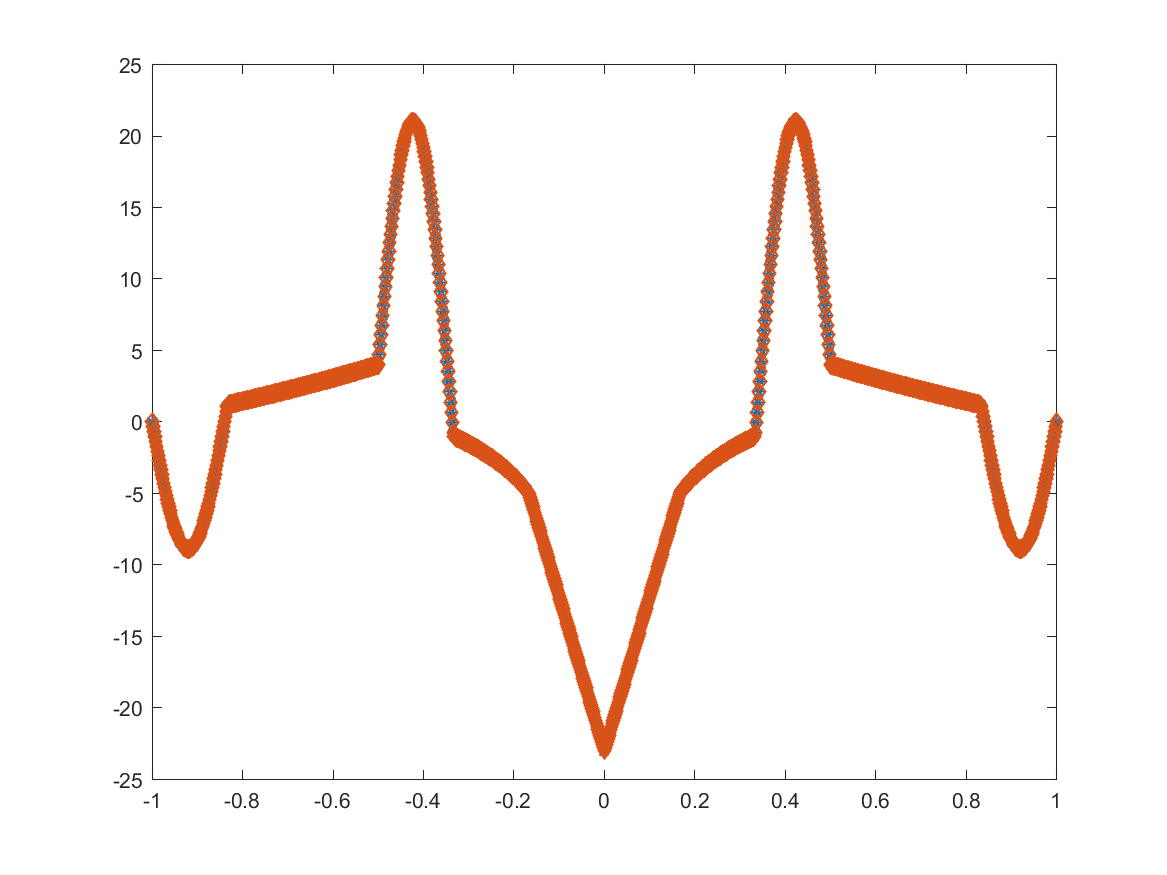
\includegraphics[width=\linewidth]
        {pictures/experiments/settings/f01/rhsAxis.png}
      \caption*{$f$ for $\alpha=1$ along the axes}
    \end{subfigure}
  \end{figure}
\end{frame}

\begin{frame}
  Then the solution to the continuous problem with input signal $f$ is given by
  $u\in H^1_0(\Omega)$ defined by $u(x)=\tilde{u}(|x|)$ for all $x\in\Omega$
  with 
  \begin{align*}
    \tilde{u}(r)\coloneqq
    \begin{cases}
      1 & \text{if } 0\leq r\leq\frac{1}{6},\\
      6r & \text{if } \frac{1}{6}\leq r\leq\frac{1}{3},\\
      2 &\text{if } \frac{1}{3}\leq r\leq\frac{1}{2},\\
      5-6r &\text{if } \frac{1}{2}\leq r\leq\frac{5}{6},\\
      0 &\text{if } \frac{5}{6}\leq r.
    \end{cases}
  \end{align*}
  
  \begin{figure}[!ht]
    \centering
    \begin{subfigure}{.4\linewidth}
      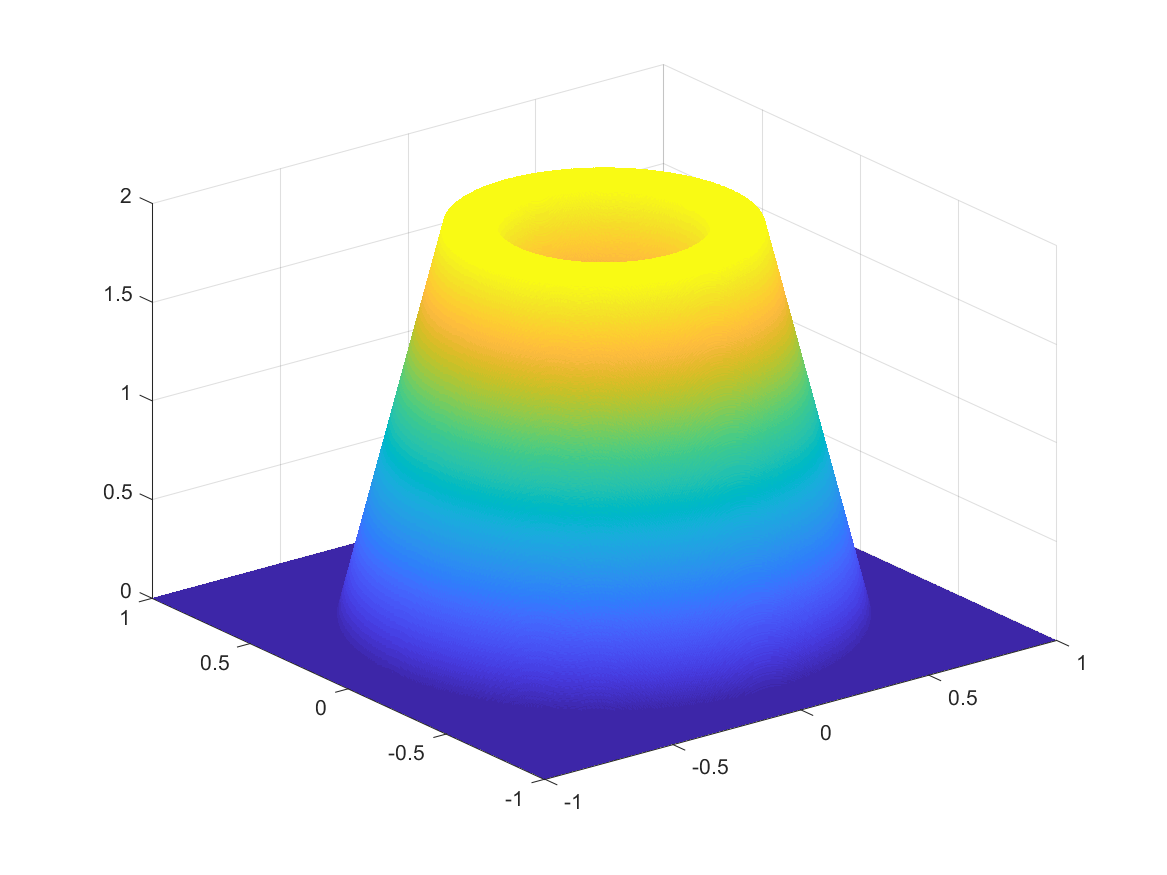
\includegraphics[width=\linewidth]
        {pictures/experiments/settings/f01/exactSolution.png}
      \caption*{$u$}
    \end{subfigure}
    \quad
    \begin{subfigure}{.4\linewidth}
      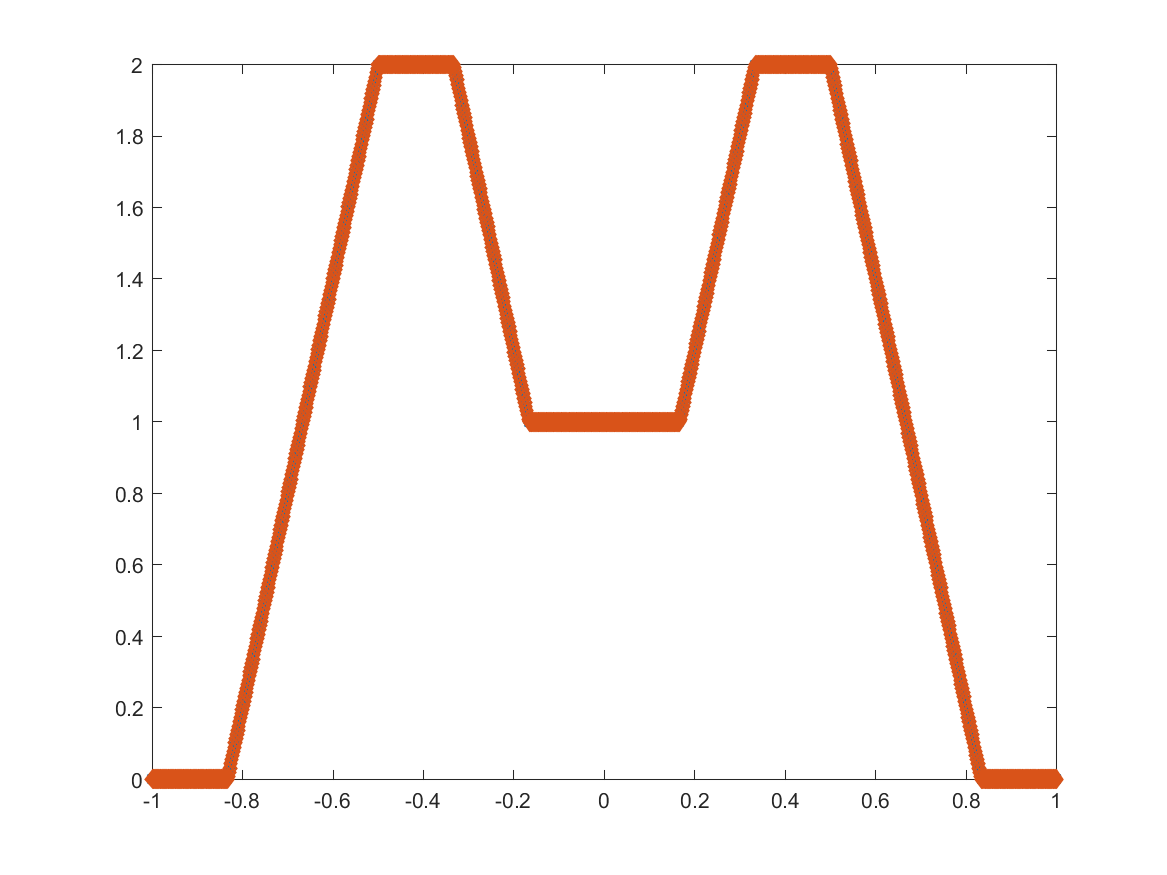
\includegraphics[width=\linewidth]
        {pictures/experiments/settings/f01/exactSolutionAxis.png}
      \caption*{$u$ along the axes}
    \end{subfigure}
  \end{figure}

  \pause
  It holds $E(u)\approx -2.058034062391$.
\end{frame}


\begin{frame}
  For $\alpha = 10000$ let the input signal represent the grayscale of an image
  in $[0,1]^{256\times 256}$ multiplied with $\alpha$ scaled to the domain
  $\Omega=(0,1)^2$.

  \begin{figure}[!ht]
    \centering
    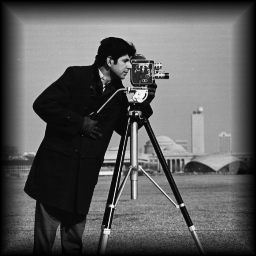
\includegraphics[width=.5\linewidth]
      {pictures/experiments/settings/images/f2bcameraman.png}
    \caption*{Image cameraman}
  \end{figure}
\end{frame}

\begin{frame}{Initial Triangulations for the Input Signals}
  \begin{figure}[!ht]
    \centering
    \begin{subfigure}{.45\linewidth}
      \caption*{Input signal $f$}
      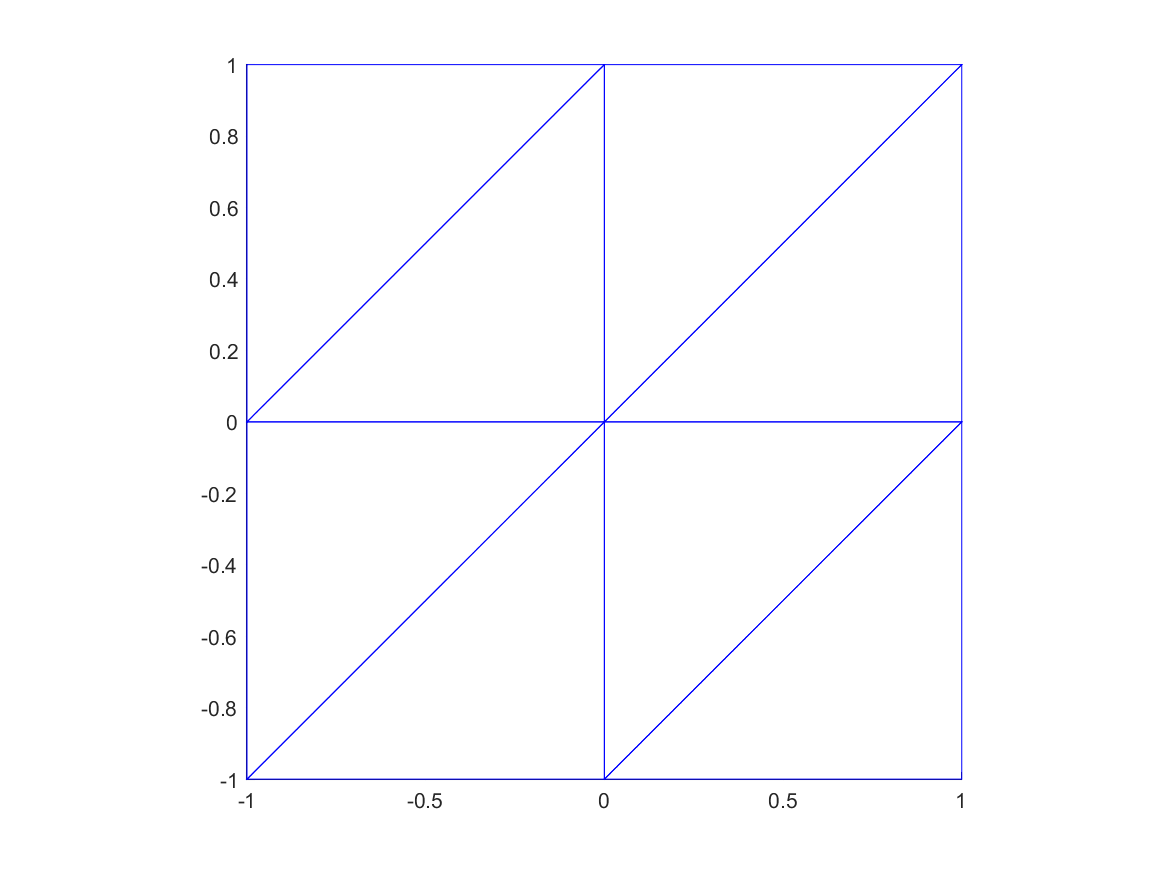
\includegraphics[width=\linewidth]
        {pictures/experiments/settings/f01/triangulation.png}
      \caption*{$\Omega = (-1,1)^2$}
    \end{subfigure}
    \begin{subfigure}{.45\linewidth}
      \caption*{Input signal cameraman}
      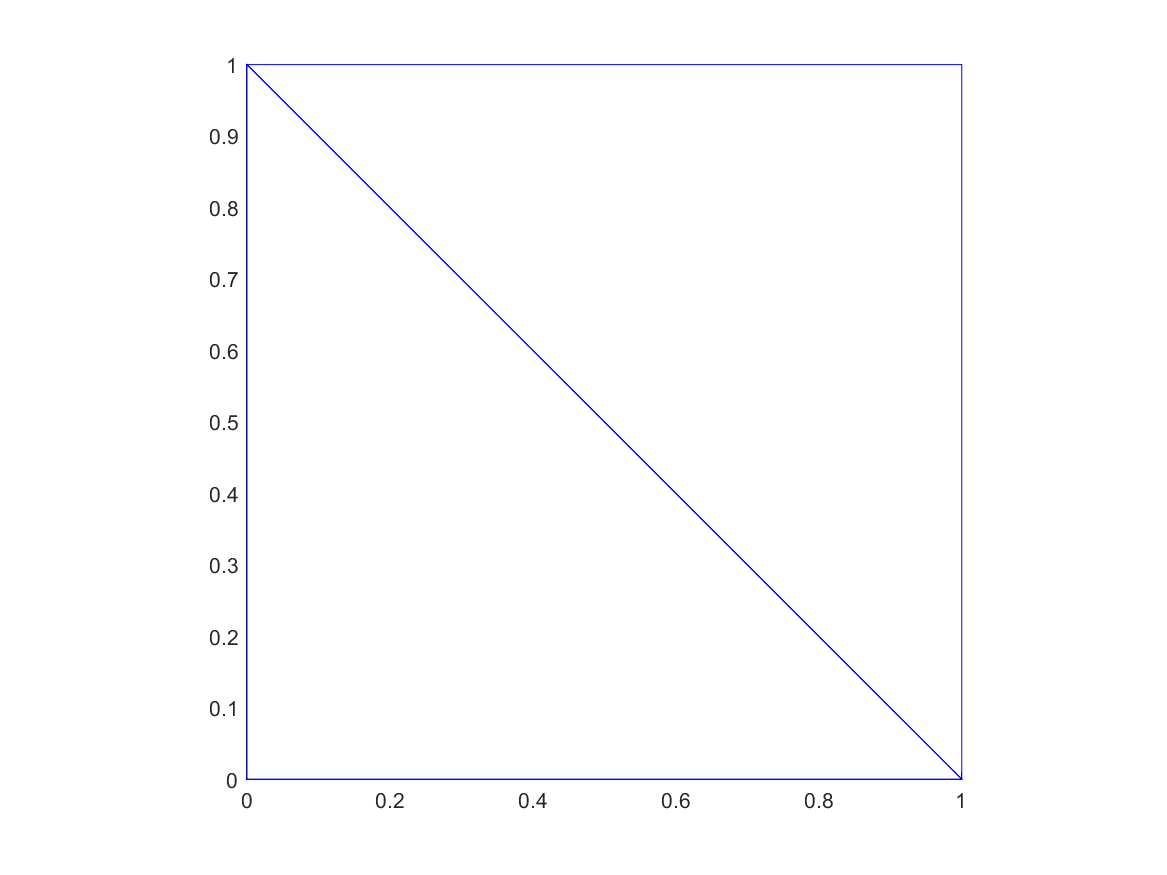
\includegraphics[width=\linewidth]
        {pictures/experiments/settings/images/triangulation.png}
      \caption*{$\Omega = (0,1)^2$}
    \end{subfigure}
  \end{figure}
\end{frame}

\subsection{Choice of Parameters}
\begin{frame}[noframenumbering]{Table of Contents}
  \tableofcontents[currentsection, currentsubsection]
\end{frame}

\begin{frame}{Choice of $\tau$}
  For the rest of the presentation (unless otherwise specified) let the bulk
  parameter be $\theta = 0.5$, and $\varepsilon_\textup{stop}= 10^{-4}$.
  \only<1>{
  \begin{figure}[!ht]
    \centering
    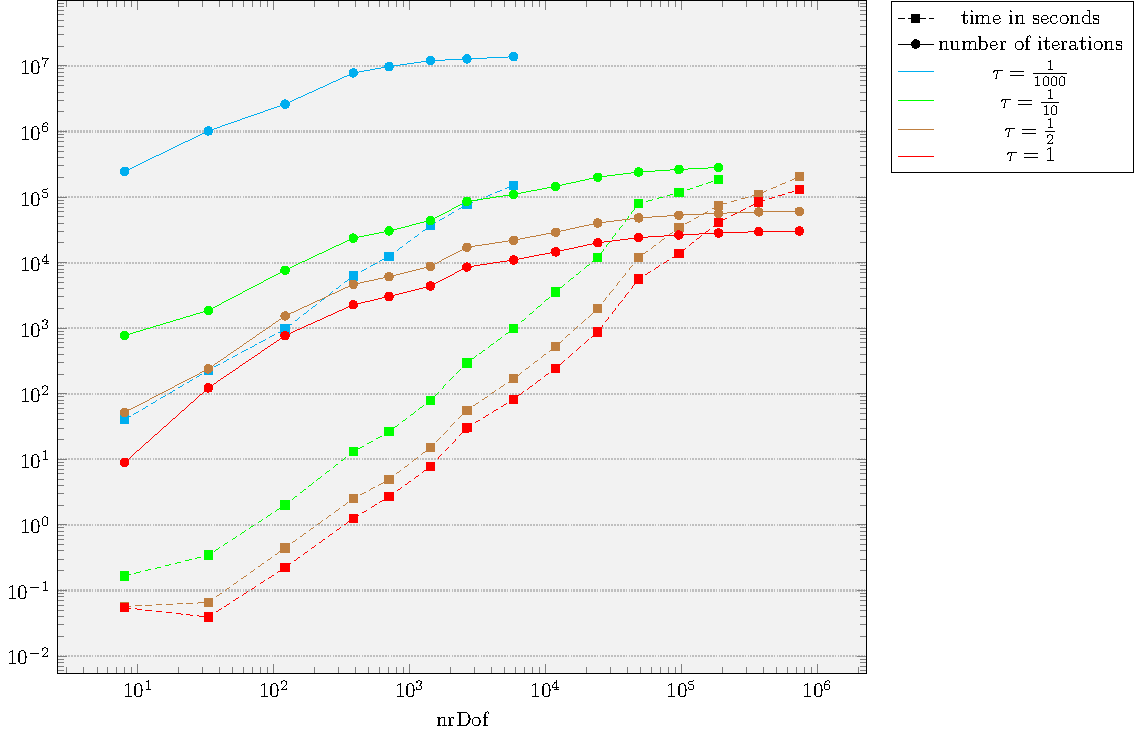
\includegraphics[width=0.9\linewidth]
      {pictures/experiments/choiceOfParameters/tau/miscF.pdf}
    \caption*{Input signal $f$}
  \end{figure}}
  \only<2>{
  \begin{figure}[!ht]
      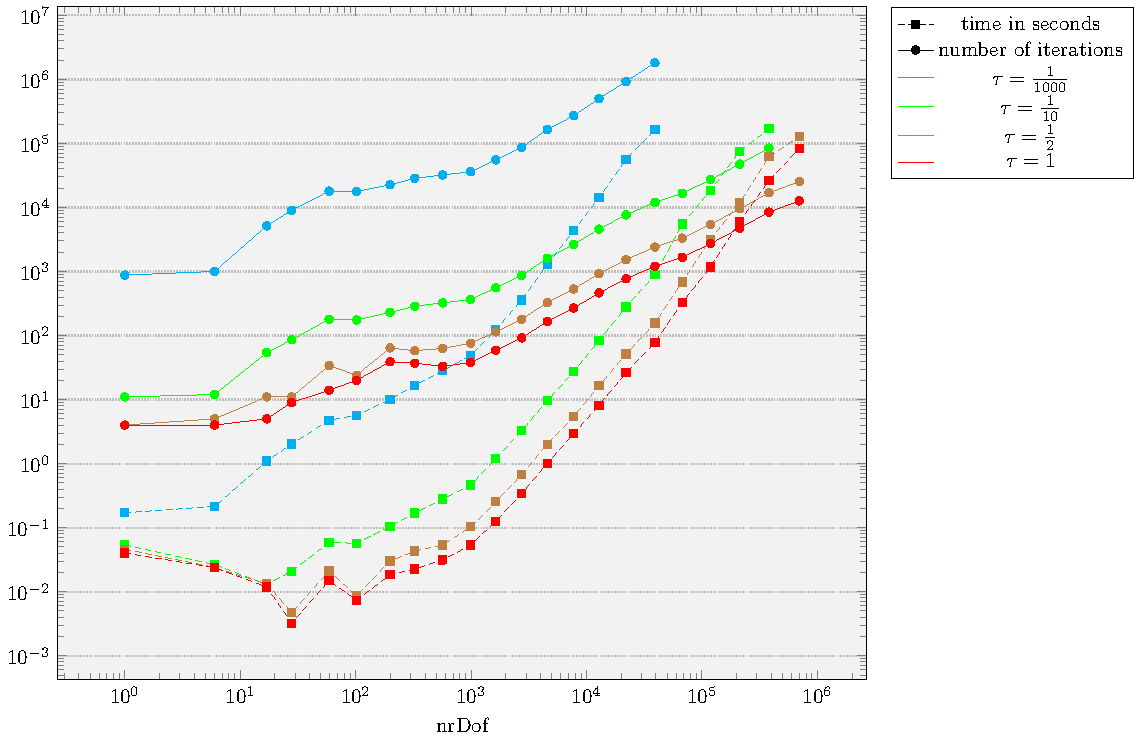
\includegraphics[width=0.9\linewidth]
        {pictures/experiments/choiceOfParameters/tau/miscCam.pdf}
      \caption*{Input signal camerman}
  \end{figure}}
  \only<3>{
  \begin{figure}[!ht]
      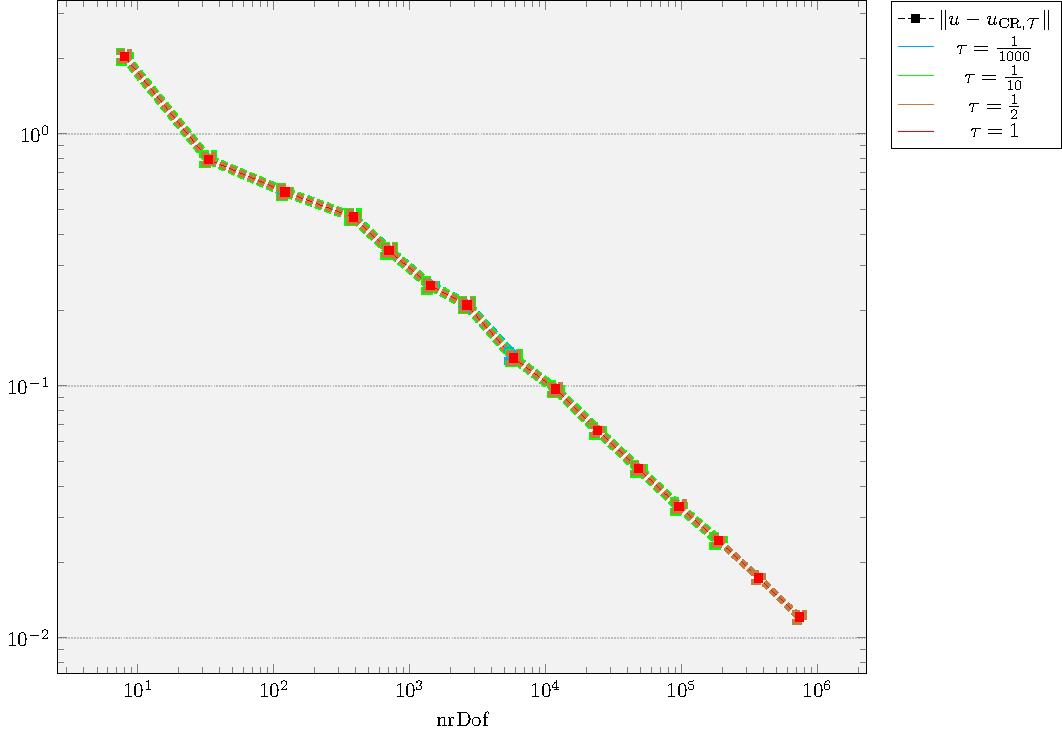
\includegraphics[width=0.8\linewidth]
        {pictures/experiments/choiceOfParameters/tau/convergenceF.pdf}
      \caption*{Input signal $f$}
  \end{figure}}
\end{frame}

\begin{frame}{Conclusion and Hypothesis}
  For the rest of the presentation $\tau = 1$.

  \pause
  \medskip
  
  Convergence of the iterates of the primal-dual iteration to the discrete
  solution $\ucr$ followed from
  \begin{align*}
    \sum_{j=1}^\infty\Vert \ucr-u_j\Vert^2 
    \leq
    \frac{1}{2\alpha{\color<3>{red}{\tau}}}
    \left({\color<5->{red}{\vvvert \ucr-u_0\vvvert^2_\nc}}
    + \Vert \bar\Lambda_0-\Lambda_0\Vert^2\right).
  \end{align*}

  \pause
  \pause
  Settings with $\tau = 1.2$ and no convergence were observed.
  \pause
  \pause

  \medskip
  For $\vcr\in\CR^1_0(\Tcal)$, define $J_1:\CR^1_0(\Tcal)\to P_1(\Tcal)\cap
  C_0(\Omega)$ by
  \begin{align*}
    J_1\vcr(z)\coloneqq |\Tcal(z)|^{-1}\sum_{T\in\Tcal(z)}\vcr|_T(z)
    \quad\text{for all }z\in\Ncal(\Omega).
  \end{align*}

  \pause

  Use $\hat u_0 \coloneqq J_1 u_{\textup{CR},\Tcal}\in P_1(\Tcal)\cap
  C_0(\Omega)\subseteq P_1\big(\hat\Tcal\big)\cap C_0(\Omega)
  \subseteq \CR^1_0\big(\hat\Tcal\big)$ as input for the iteration on the
  refined triangulation $\hat\Tcal$.
\end{frame}

\begin{frame}{Choice of $\varepsilon_\textup{stop}$}
  With $\tau=1$ the stopping criterion reads $\vvvert u_j-u_{j-1}\vvvert_\nc<
  \varepsilon_\textup{stop}.$
  \begin{figure}[!ht]
    \centering
    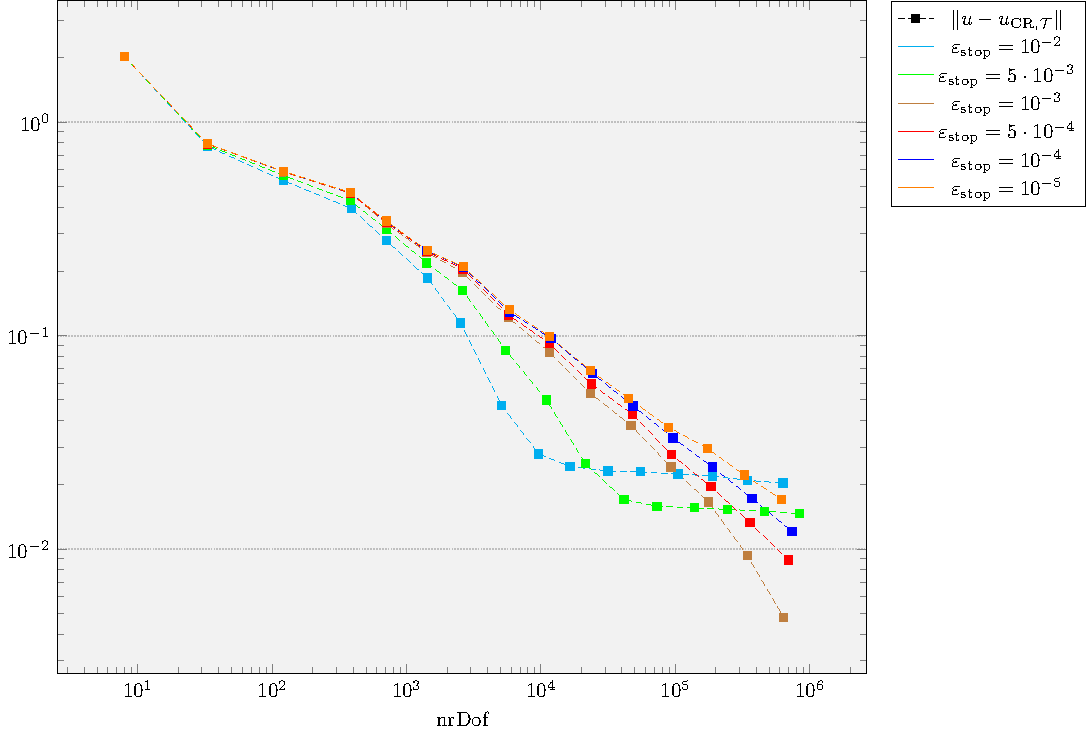
\includegraphics[width=0.8\linewidth]
      {pictures/experiments/choiceOfParameters/epsStop/convergence.pdf}
  \end{figure}

  \pause
  For the rest of the presentation $\varepsilon_\textup{stop} = 10^{-4}$.
  %$\vvvert\bullet\vvvert_\nc \approx h^{-1}\Vert\bullet\Vert$.
\end{frame}


\subsection{Guaranteed lower Energy Bound and Refinement Indicator}
\begin{frame}[noframenumbering]{Table of Contents}
  \tableofcontents[currentsection, currentsubsection]
\end{frame}

\begin{frame}
  \begin{theorem}[Guaranteed lower energy bound]
    Let $\Omega$ be convex. Let $f\in H^1_0(\Omega)$ be the input signal of the
    continuous (discrete) problem with solution $u\in H^1_0(\Omega)$ ($\ucr\in
    \CR^1_0(\Omega)$).
    Then
    \begin{align*}
      \Enc(\ucr)+\frac{\alpha}{2}\Vert u-\ucr\Vert^2
      -\frac{\kappa_\CR}{\alpha}\Vert
      h_\Tcal(f-\alpha\ucr)\Vert \Vert\nabla f\Vert\leq E(u)
    \end{align*}
    with $\kappa_\CR\coloneqq\sqrt{1/48+1/j_{1,1}^2} \approx 0.298217419$.
    \pause
    In particular 
    \begin{align*}
      \Egleb 
      \coloneqq 
      \Enc(\ucr) - \frac{\kappa_\CR}{\alpha}\Vert h_\Tcal(f-\alpha\ucr)\Vert
      \Vert \nabla f\Vert
    \end{align*}
      satisfies $\Enc(\ucr)\geq \Egleb$ and $E(u)\geq \Egleb$.
  \end{theorem}
\end{frame}


\begin{frame}
  \begin{definition}[Refinement indicator]
    Let $0<\gamma\leq 1$ (in this presentation $\gamma=1$).
    For all $T\in\Tcal$ and $\ucr\in\CR^1_0(\Tcal)$, define
    \begin{align*}
      \eta_\text{V}(T)
      &\coloneqq
      |T|\Vert f-\alpha \ucr\Vert^2_{L^2(T)},\\
      \eta_\text{J}(T)
      &\coloneqq |T|^{\gamma/2}\sum_{F\in\Ecal(T)}\left\Vert
      [\ucr]_F\right\Vert_{L^1(F)},\quad\text{and }\\
      \eta (T)
      &\coloneqq
      \eta_\text{V}(T) + \eta_\text{J}(T).
    \end{align*} 
    With that define the refinement indicator
    $\eta\coloneqq\sum_{T\in\Tcal}\eta(T)$.
  \end{definition}
\end{frame}

\DTLloaddb{db}
{pictures/experiments/refIndTriang/cam/lvl16/currentDataReduced.csv}
%\DTLassign{db}{1}{\nrNodesZe=nrNodes, \nrDofZe=nrDof}
\DTLassign{db}{1}{\nrDof=nrDof}
\DTLgdeletedb{db}

\begin{frame}
  The mesh with \nrDof\ degrees of freedom for level 16 of the adaptive
  algorithm with $\theta = 0.5$ and input signal cameraman and the solution of
  the iteration on this mesh.

  \begin{figure}[!ht]
    \centering
    \begin{subfigure}{.6\linewidth}
      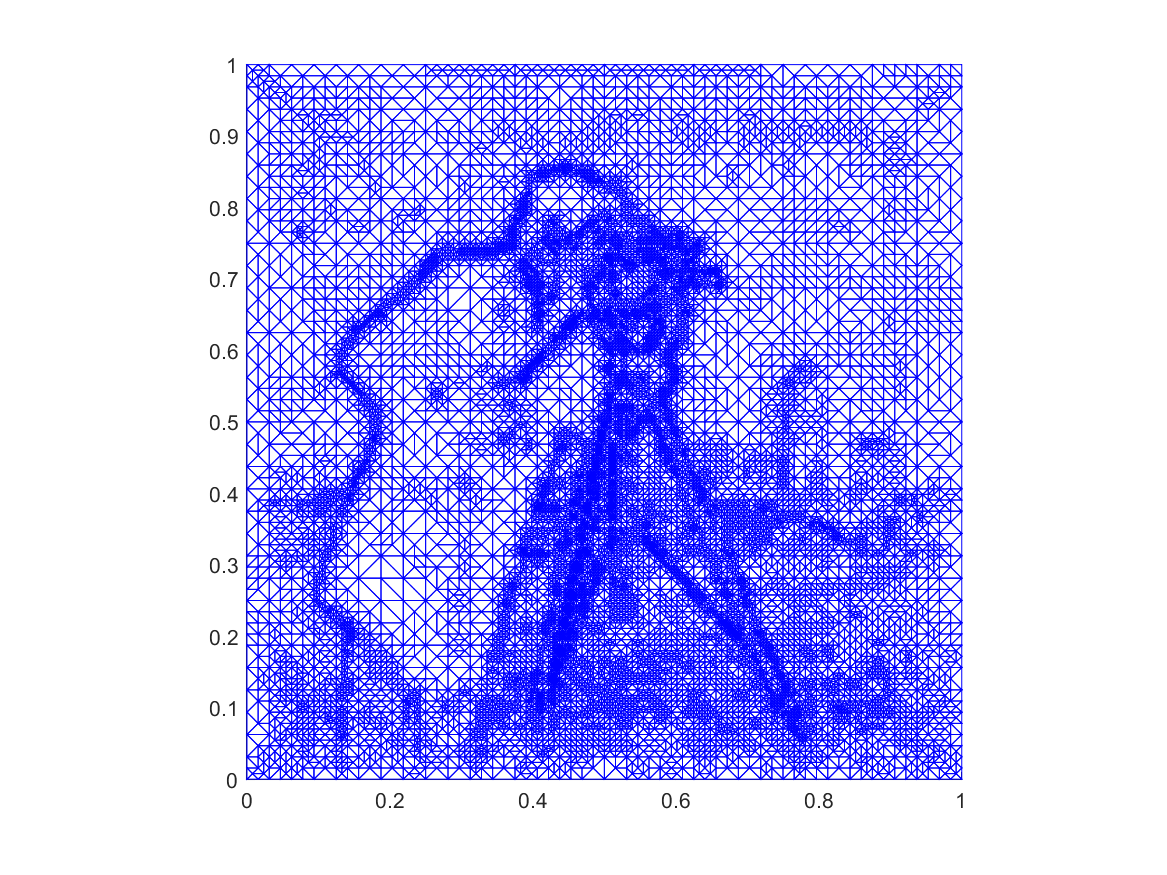
\includegraphics[trim = 100 30 20 20, clip,width=\linewidth]
        {pictures/experiments/refIndTriang/cam/lvl16/triangulation.png}
    \end{subfigure}
    \hspace{-1.2cm}
    \begin{subfigure}{.4\linewidth}
      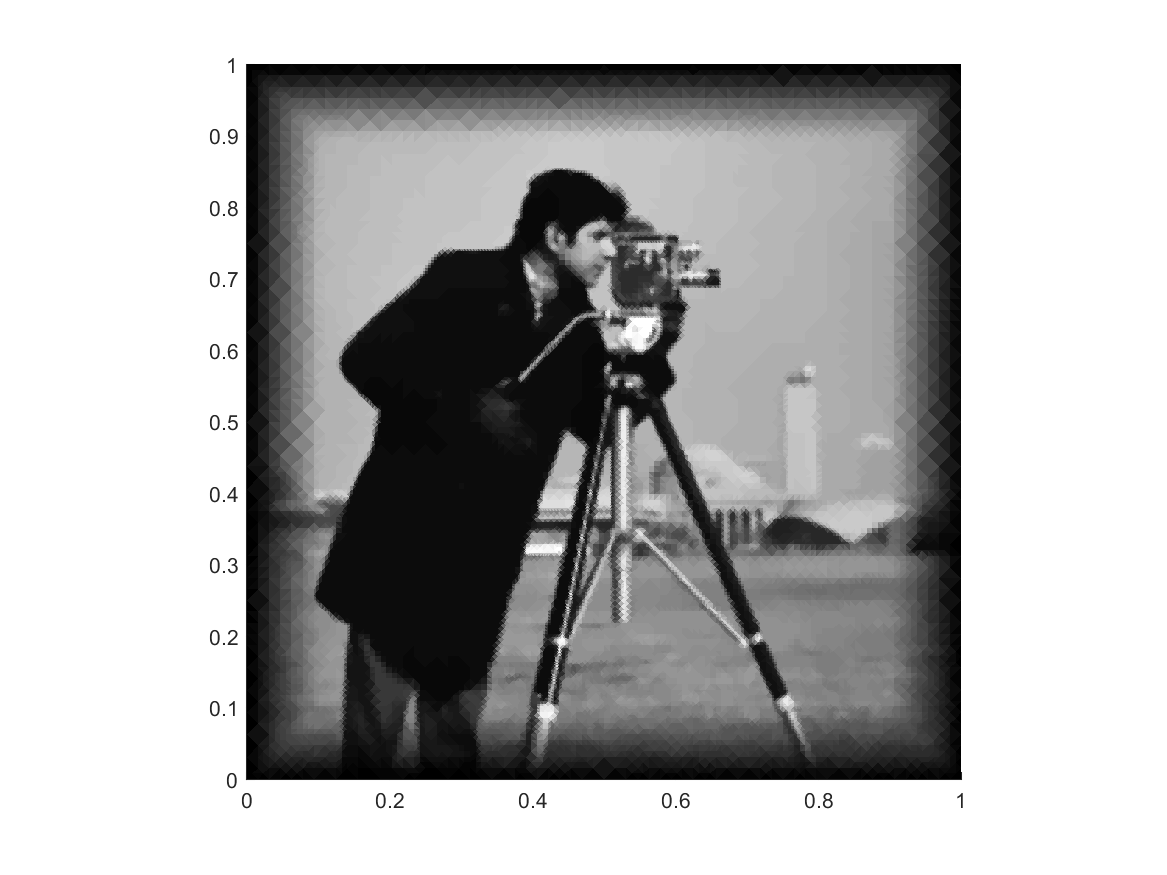
\includegraphics[trim = 80 30 80 20, clip, width=\linewidth]
        {pictures/experiments/refIndTriang/cam/lvl16/solutionGrayscale.png}
    \end{subfigure}
  \end{figure}
\end{frame}

\DTLloaddb{db}
{pictures/experiments/refIndTriang/f01/lvl11/currentDataReduced.csv}
%\DTLassign{db}{1}{\nrNodesZe=nrNodes, \nrDofZe=nrDof}
\DTLassign{db}{1}{\nrDof=nrDof}
\DTLgdeletedb{db}

\begin{frame}
  The mesh with \nrDof\ degrees of freedom for level 11 of the adaptive
  algorithm with $\theta = 0.5$ and input signal $f$ and the solution of the
  iteration on this mesh along the axes.

  \begin{figure}[!ht]
    \centering
    \begin{subfigure}{.6\linewidth}
      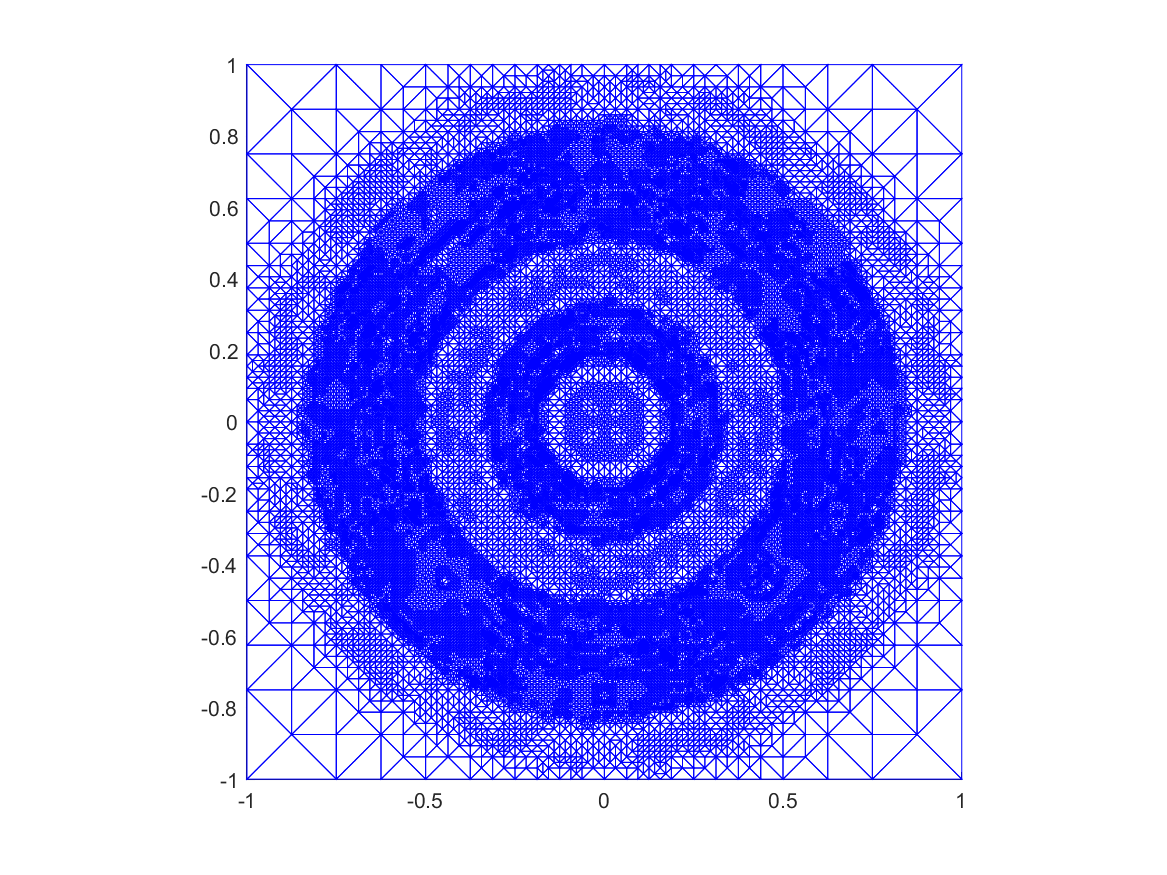
\includegraphics[trim = 100 30 20 20, clip,width=\linewidth]
        {pictures/experiments/refIndTriang/f01/lvl11/triangulation.png}
    \end{subfigure}
    \hspace{-1.2cm}
    \begin{subfigure}{.4\linewidth}
      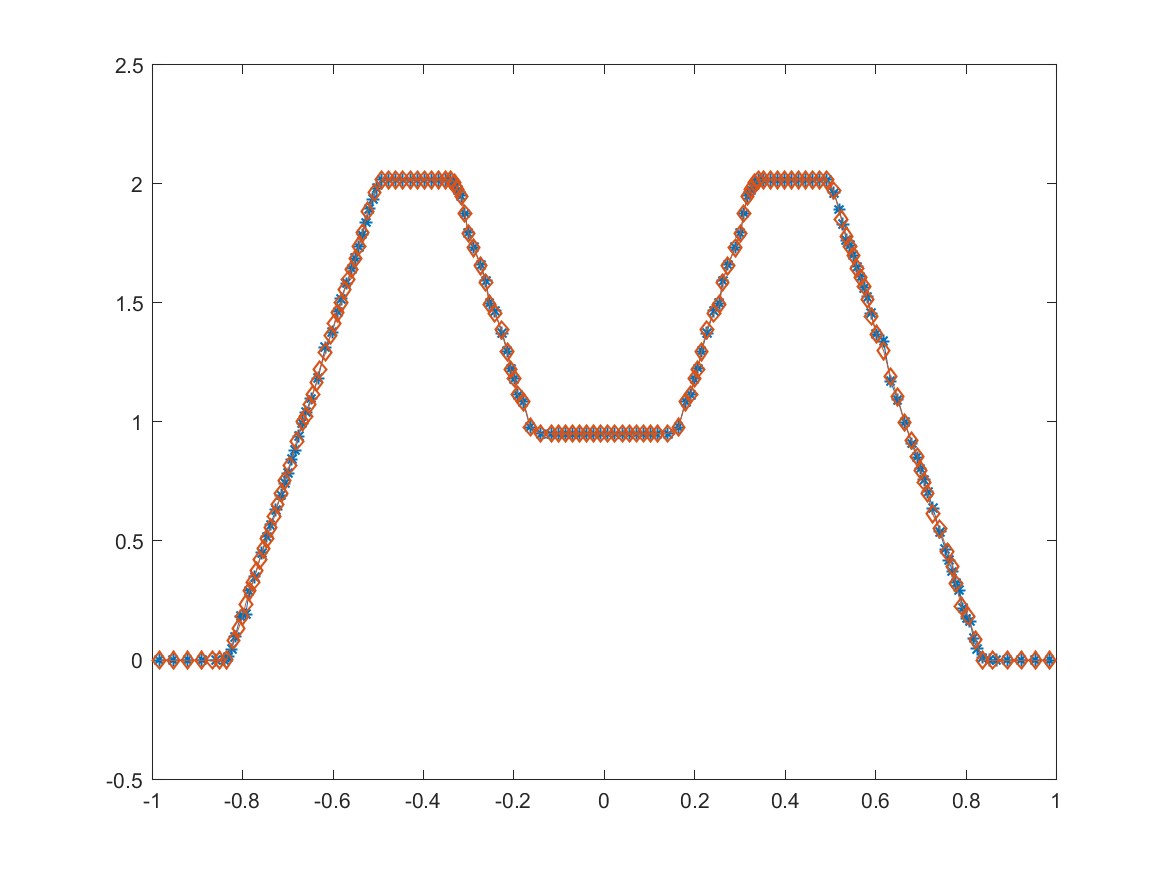
\includegraphics[trim = 50 30 50 20, clip, width=\linewidth]
        {pictures/experiments/refIndTriang/f01/lvl11/solutionAxis.png}
    \end{subfigure}
  \end{figure}
\end{frame}

\begin{frame}
  \begin{figure}[!ht]
    \centering
    \begin{subfigure}{.49\linewidth}
      \caption*{Input signal $f$}
      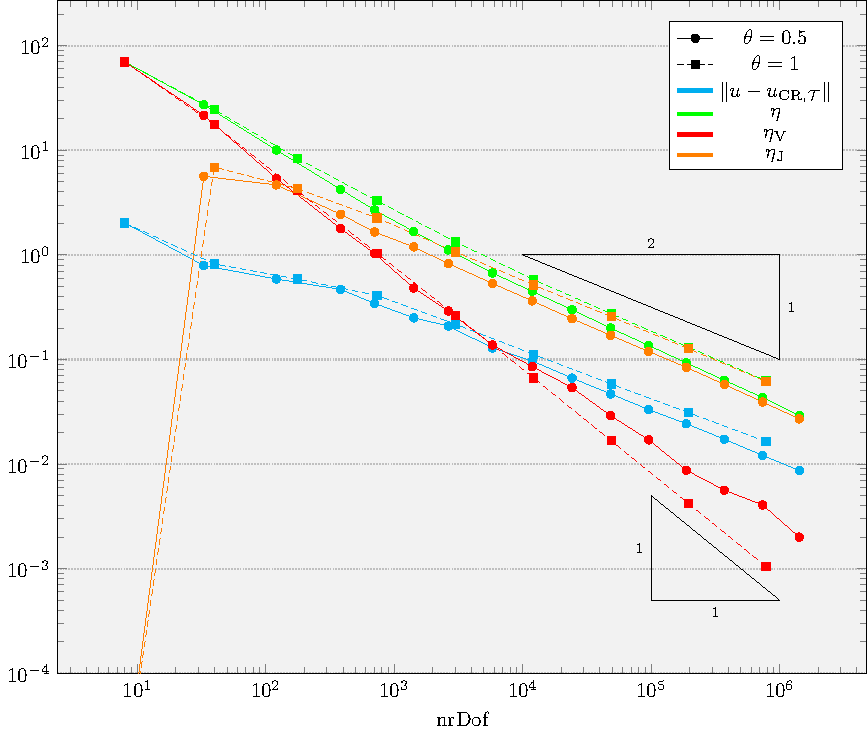
\includegraphics[width=\linewidth]
        {pictures/experiments/refIndGlebConvergence/f01/convergenceEtaError.pdf}
    \end{subfigure}
    \begin{subfigure}{.49\linewidth}
      \caption*{Input signal cameraman}
      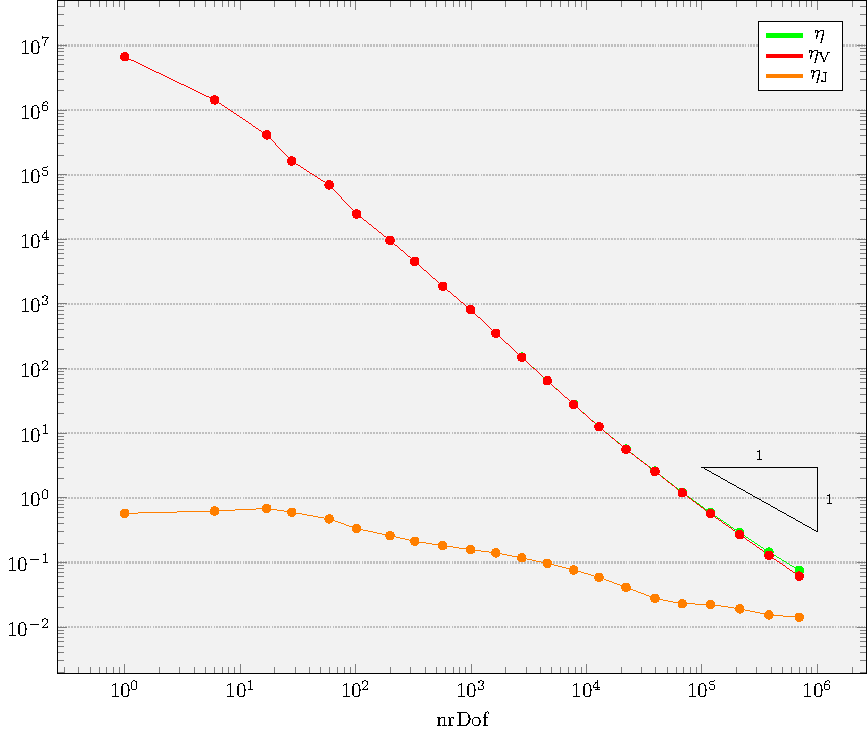
\includegraphics[width=\linewidth]
        {pictures/experiments/refIndGlebConvergence/cam/convergenceEta.pdf}
    \end{subfigure}
  \end{figure}

  \pause
  \vspace{-0.5cm}
  \begin{block}{\cite[p. 309, Thm. 10.7]{Bar15}}
    For the conforming discretization of the ROF model problem with the 
    Courant FEM it holds
    \begin{align*}
      \frac{\alpha}{2}\Vert u-u_\text{C}\Vert^2\lesssim h^{1/2}. 
    \end{align*}
  \end{block}
\end{frame}

\begin{frame}
  \begin{figure}[!ht]
    \centering
    \caption*{Input signal f}
    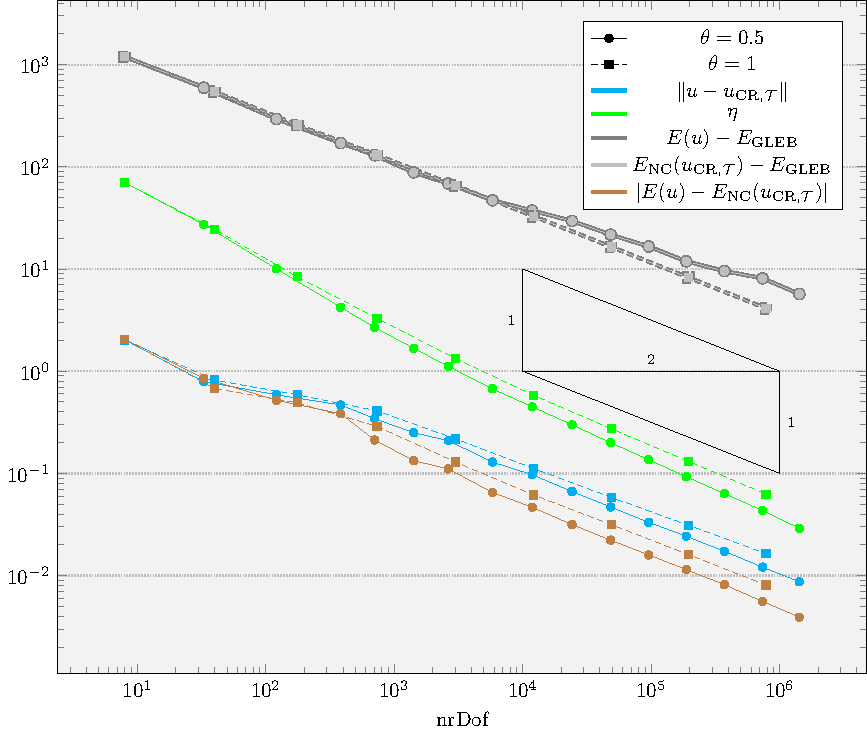
\includegraphics[width=0.8\linewidth]
        {pictures/experiments/refIndGlebConvergence/f01/convergenceEtaErrorGleb.pdf}
  \end{figure}
\end{frame}

\begin{frame}
  \begin{block}{ }
    Let $u\in\BV(\Omega)\cap L^2(\Omega)$ ($\ucr\in\CR^1_0(\Tcal)$) solve the
    continuous (discrete) problem with input signal $f$.
    Then
    \begin{align*}
      \frac{\alpha}{2}\Vert u-\ucr\Vert^2
      &\leq
      E(\ucr)-E(u)\\
     &=
      \Enc(\ucr)+\sum_{F\in\Ecal}\Vert[\ucr]_F\Vert_{L^1(F)}-E(u).
    \end{align*}
  \end{block}

  \pause
  \begin{figure}[!ht]
    \centering
    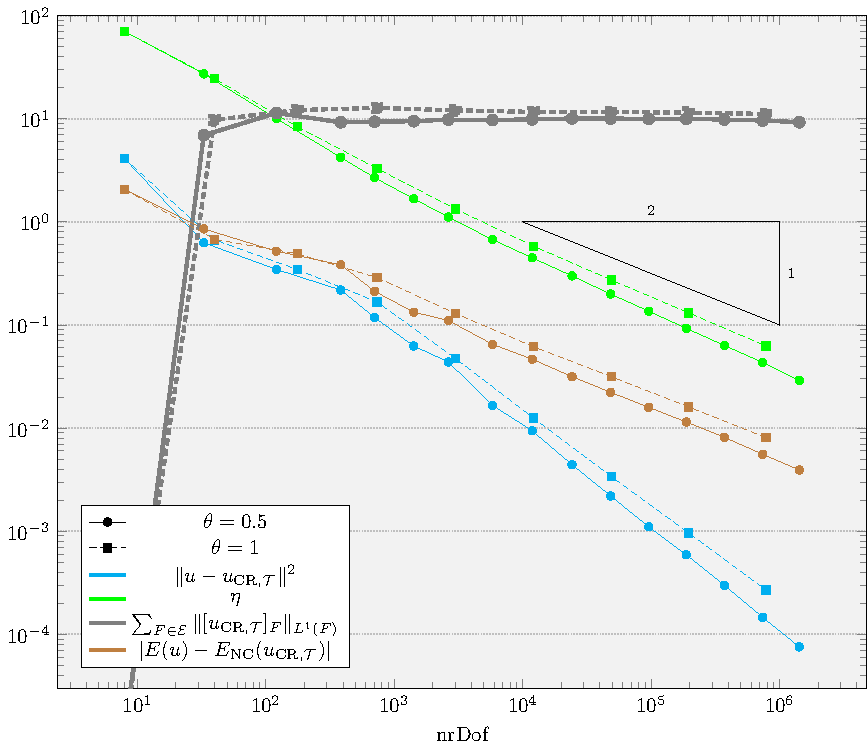
\includegraphics[width=0.5\linewidth]
        {pictures/experiments/refIndGlebConvergence/f01/convergenceEtaErrorSquGleb.pdf}
        \caption*{Input signal f}
  \end{figure}
\end{frame}

\subsection{Convergence of the Iteration} 
\begin{frame}[noframenumbering]{Table of Contents}
  \tableofcontents[currentsection, currentsubsection]
\end{frame}

\begin{frame}{Input Signal $f$, $\theta = 0.5$}
  \only<1>{
  \begin{figure}[!ht]
    \centering
    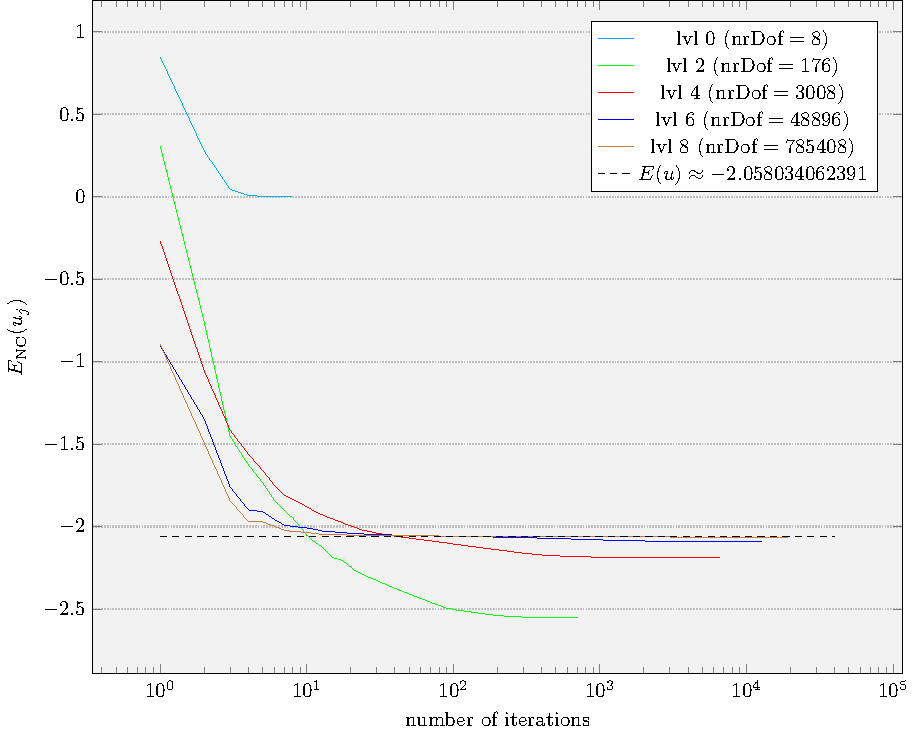
\includegraphics[width=0.8\linewidth]
      {pictures/experiments/convergenceIteration/convergenceIteration.pdf}
      \caption*{$\tau = 1$}
  \end{figure}}
  \only<2>{
  \begin{figure}[!ht]
      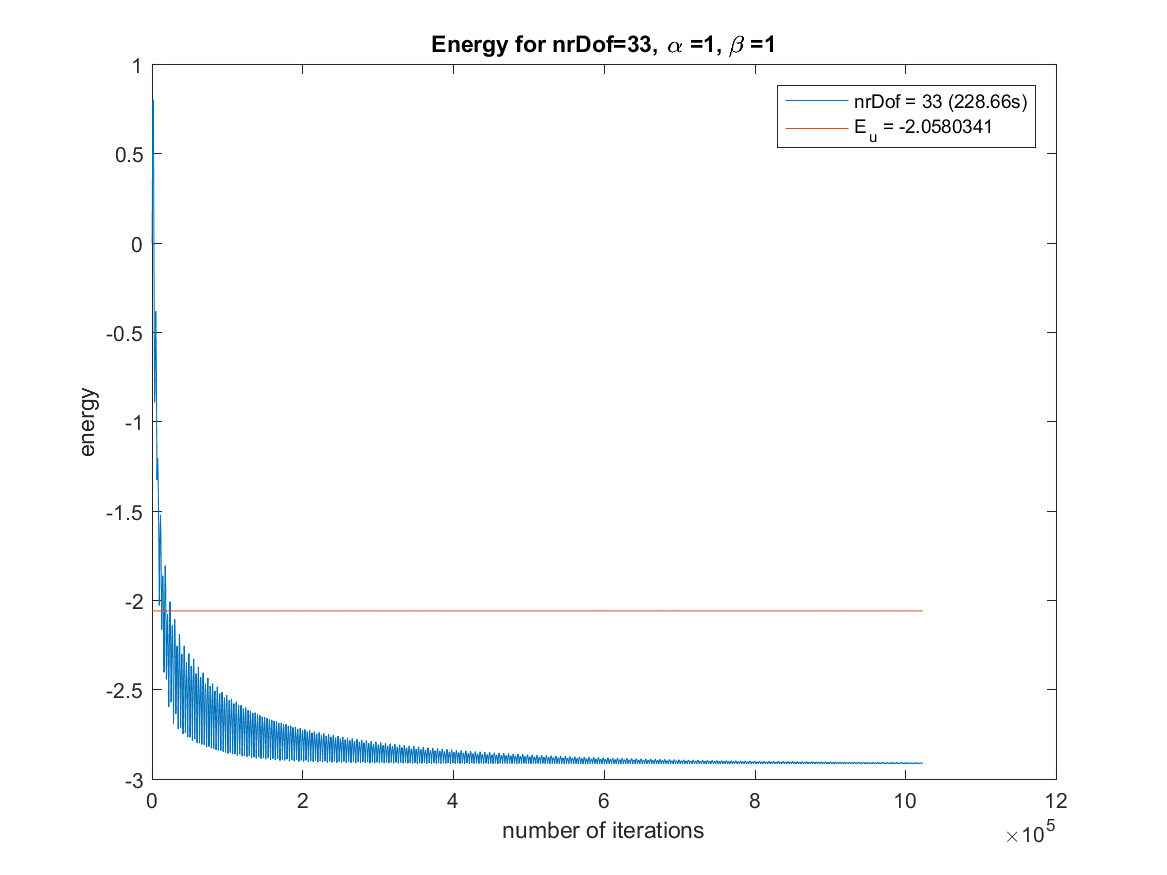
\includegraphics[width=0.9\linewidth]
        {pictures/experiments/convergenceIteration/f01TauTiny.png}
       \caption*{$\tau = 10^{-3}$}
  \end{figure}}
\end{frame}
